\renewcommand{\chaptername}{Selección de hardware para implementación del sistema} 
\graphicspath{{parte_1/cap3/}}
\chapter{Selección de hardware para implementación del sistema} \label{cap:cap3_sel_hw}
\markright{\chaptername }
\begin{center}
\begin{tcolorbox}[colback=gray!5!white, %Color del fondo
colframe=blue!75!black,
title= \center{\Large{resumen}} ]
Aquí, definimos algunos de los componentes de hardware seleccionados para cumplir con los requerimientos, en particular, definimos el microcontrolador, la interfaz de red, y la interfaz de usuario del sistema. En esta sección, el análisis se basa sobre componentes disponibles en el IAR, de estos, seleccionamos aquellos, que cumplen el requisito de bajo costo, y luego sobre los mismos, se analiza su facilidad de programación, librerías disponibles, módulos disponibles sobre estos, y otros aspectos.  
\end{tcolorbox}
\end{center}    

\section{Introducción} 
Se definen los criterios de selección del microcontrolador, además, se define la interfaz de red y la de usuario. Los componentes se han seleccionado en base a los siguientes criterios: 
\begin{enumerate}
  \item Compatibilidad entre las partes.  
  \item Disponibilidad de documentación para el desarrollo. 
  \item Cantidad de puertos entrada/salida de cada microcontrolador o computadora 
\end{enumerate}

Al ser una antena, que debe seguir satélites, se debe tener en cuenta, que los satélites, varían su velocidad, según el punto de la órbita en que se encuentren. Dado que esta velocidad varía, este seguimiento, debe adaptarse a estos cambios. Estos cambios son del orden de los segundos, y cualquier microprocesador actual funcionan en orden de los megahertz, con lo cual, si se realiza el control en tiempos del orden de milisegundos, el control podría realizarse sin ningún tipo de inconveniente. Por este motivo, la velocidad de la computadora, no es un factor crítico a tener en cuenta en los puntos de vista para la selección del hardware.    


\section{Componentes de hardware} \label{Sec_CompH}


La computadora, o microcontrolador, debe tener interfaces, para conectarse con el mundo exterior. El hecho es que requiere realizar la medición de dos posiciones en simultaneo, que son el ángulo de acimut y la altura. La antena, posee adosado, dos potenciómetros, que cumplen la función de encoders. Por ende, al tener adosado estos dos potenciómetros, el microcontrolador, debe tener dos canales o puertos de entrada que posean un conversor analógico-digital cada uno. 

La interfaz de red, debe ser independiente del microprocesador o controlador, para cumplir con el requerimiento de escalabilidad, por ende, se debe utilizar alguna solución integrada que se conecte al microcontrolador principal, y puedan intercambiar mensajes entre ellos. 

La interfaz para el estado de la antena, se usará una pantalla, la cual mostrará el estado de la misma. Para ello, se usará un display LCD de 16x2 que se encuentra disponible para su uso.


De lo expuesto en los párrafos anteriores, el microcontrolador, debe ser independiente de todo el hardware asociado. Además debe poseer una electrónica asociada a cada motor, que permita encender o apagar cada motor de forma independiente. Además, debe ser capaz de controlar el sentido de giro de cada motor. Dado que estas maniobras las debe realizar el microcontrolador, se requieren de al menos cuatro puertos disponibles sobre el microcontrolador(dos puertos para cada motor, y con un único puerto, se selecciona el sentido de giro). 


\subsection{Interfaz de red - Materiales disponibles}\label{Int_r} 

La placa disponible en el IAR, es la siguiente: chip Ethernet W5100. Las misma se muestra a continuación. 

\begin{figure}[ht]
	\centering	
	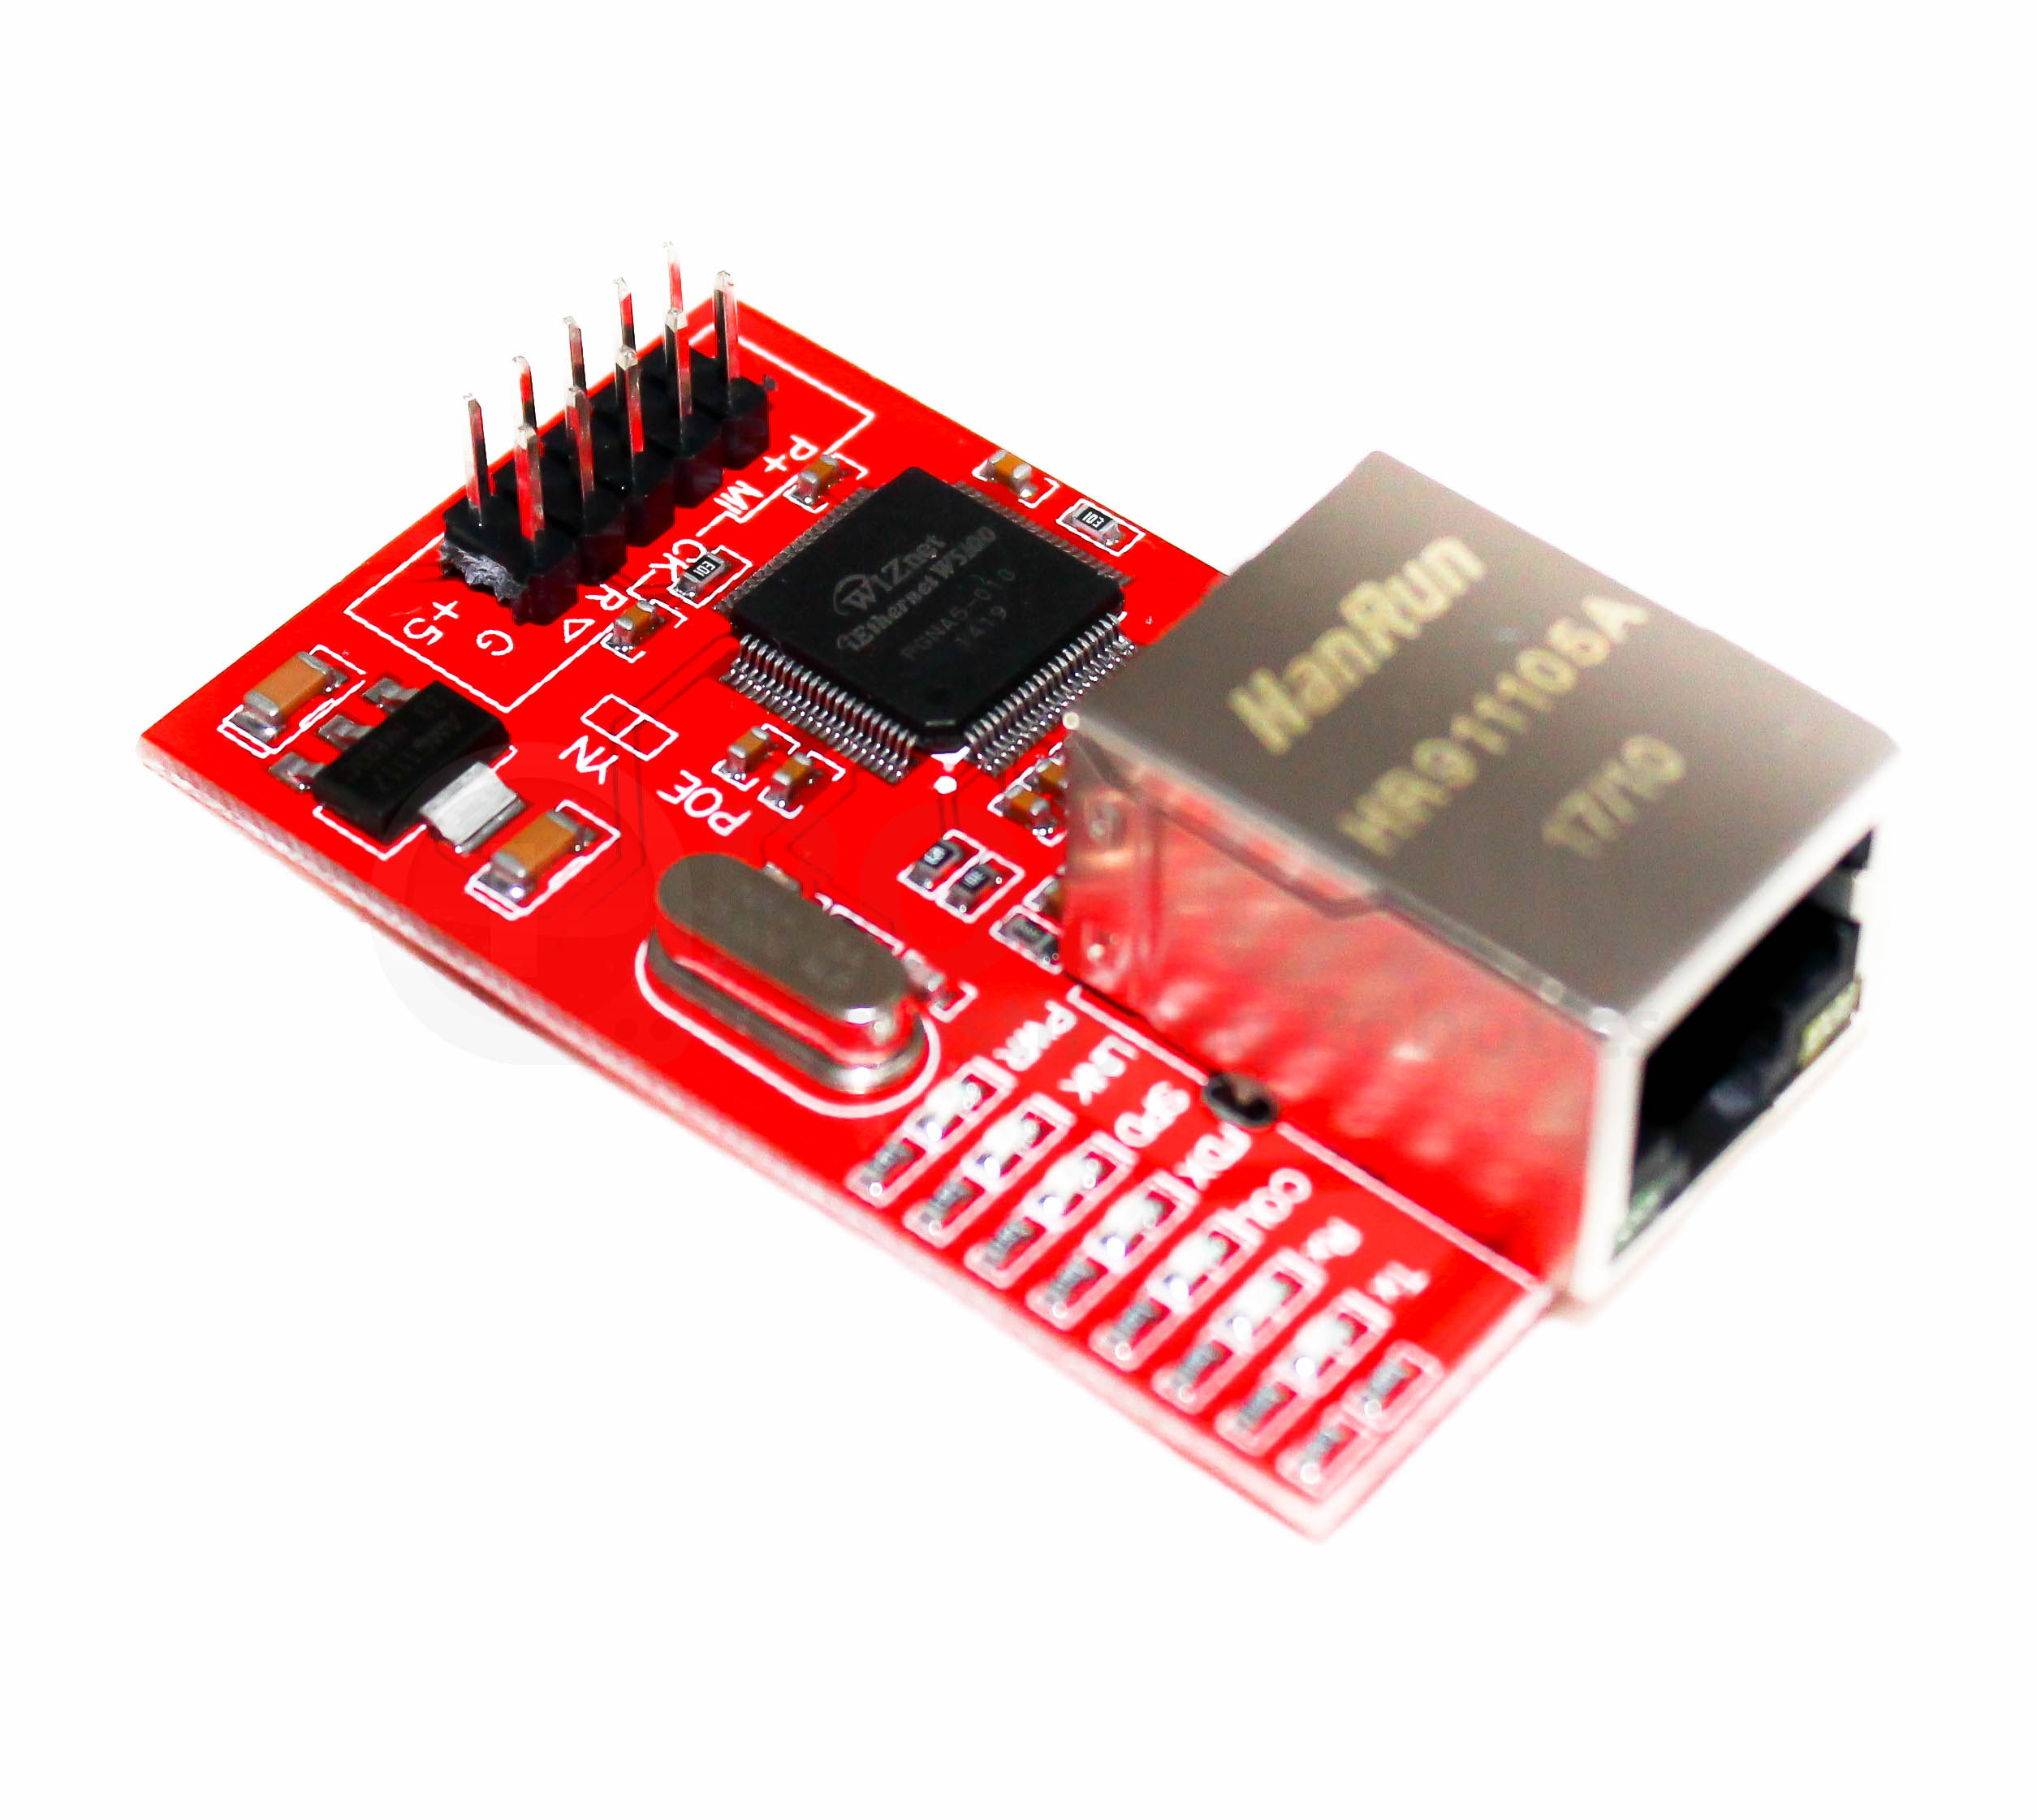
\includegraphics[scale=.2]{w5100}  
	\caption{Chip Ethernet W5100}		 
	%\caption{dispositivos disponibles IAR} 
	\label{fig:chip_ethernet}
\end{figure}

La placa ethernet W5100(ver figura \ref{fig:chip_ethernet}) es un controlador dedicado a las redes. Al recibir un dato, este lo transmite, mediante un puerto paralelo, o por puerto SPI(serial paralell interface). Cabe destacar, que este desarrollo, solo tiene disponible el bus SPI, ya que la placa, solo viene con este protocolo. Además, esta placa, no puede compartir el bus, debido a el diseño de la misma. Si desea compartir el bus, debe modificarse. Uno de los requerimientos es que no debe utilizar redes inalámbricas, por este motivo, se utiliza esta interfaz de red. 

\subsection{Interfaz de usuario} \label{Int_u}
% explicacion display por I2C 
Como se expuso en la sección \ref{Sec_CompH}, se va a utilizar un display LCD de 16 columnas y 2 filas,que está disponible para su uso en el Instituto Argentino de Radioastronomía.  
 
El display LCD, es una pantalla, la cual es capaz de mostrar texto, valores numéricos, crear símbolos propios,etc.El display LCD disponible, se muestra en la figura \ref{fig:LCD_r}: 
\begin{figure}[ht]
	\centering
	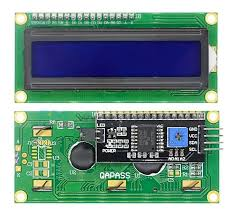
\includegraphics{dispLCD} 
	\caption{Display LCD en el IAR}
	\label{fig:LCD_r}
\end{figure}

La imagen, se ve que el display LCD, tiene adosado, un controlador, este controlador es un circuito integrado denominado PCF8574. Este dispositivo, es capaz, de expandir la cantidad de pines de un microcontrolador, utilizando el protocolo I2C. La ventaja de esto, es que a partir de dos pines se pueden controlar 8 puertos, y esto ahorra en cantidad de puertos de entrada y salida a la hora de elegir el microprocesador. Por ende, el microcontrolador seleccionado debe poseer un controlador o interfaz I2C   



\subsection{Microcontroladores disponibles}  

Los microcontroladores disponibles dentro de la institución, están embebidos dentro de placas de desarrollo, ya diseñadas, y comerciales. Por lo expuesto en las secciones anteriores(ver secciones \ref{Int_r},\ref{Int_u}),el microcontrolador seleccionado debe tener las siguientes características:

\begin{enumerate}
	\item Cantidad de conversores analógico/digital: 2
	\item Cantidad de pines disponibles: 4 (mínimo) 
	\item Puerto SPI: conexionado del chip ethernet
	\item Puerto I2C: para la conexión del display 
\end{enumerate}

 De las placas de desarrollo que hay actualmente en el IAR, se tienen las siguiente placas a analizar: 
 
\begin{enumerate}
	\item EDU-CIAA
	\item Arduino Uno 
	\item STM32VL discovery 
\end{enumerate}
Donde, de las tres, debemos elegir aquella que tenga un menor valor económico, estudiar las soluciones de software y documentación que posean, y revisar si tienen puertos SPI e I2C para el display usado como interfaz de usuario y el chip Ethernet W5100. El estudio realizado se basó en las referencias \cite{placastm32vl,arduno,eduuciaaa}  

% comparación de soluciones: 
\subsubsection{EDU-CIAA}

\begin{wrapfigure}[12]{l}[2mm]{0.4\textwidth}
	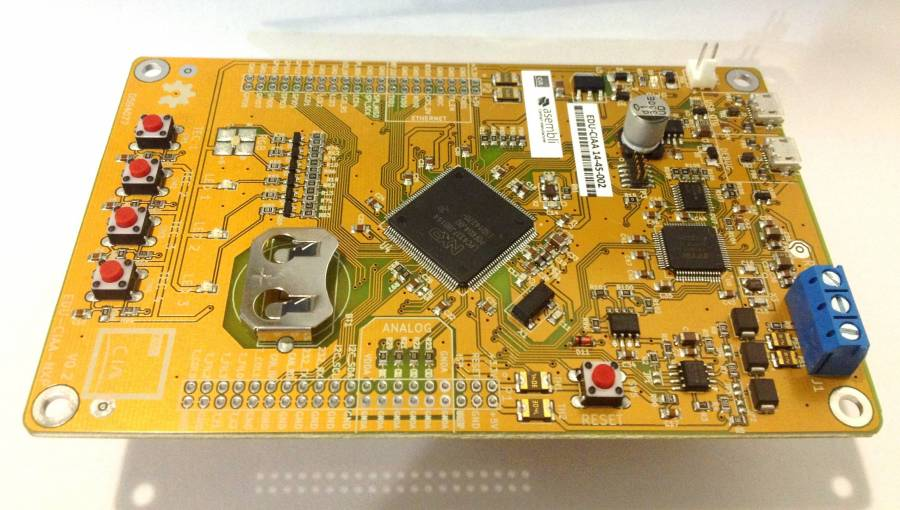
\includegraphics[width=0.4\textwidth , height=  45mm]{edu_ciaa}
	\caption{Eduu Ciaa disponible en el IAR}
	\label{fig:edu_ciaa}
\end{wrapfigure}
La placa EDU-CIAA, es una computadora de software abierto, desarrollada en argentina. Su núcleo se basa en un microprocesador cortex ARM 4.Su microcontrolador es el LPC4337. La documentación existente está incompleta. Algunas partes, están desarrolladas y otras partes, aún están en desarrollo. Posee todas las interfaces necesarias para interactuar con los demás módulos(SPI, I2C,conversores A/D y pines disponibles), se puede realizar una depuración sobre la misma placa,sobre un protocolo denominado JTAG. 


Posee un IDE, y los archivos de compilación(makefile) para cargar el código sobre esta placa. La placa se muestra en la figura \ref{fig:edu_ciaa}. La EDU-CIAA está pensada en software y hardware libre. Todos los esquemáticos de circuitos, y los componentes de software, existen disponibilidad para descargarse y modificarse libremente. 

Esta placa de desarrollo, está pensada para aprender programación sobre microcontroladores, por ende, tiene todas sus interfaces integradas sobre la placa. Posee librerías disponibles para el uso de SPI e I2C. Estas librerías, no poseen documentación, por lo tanto, deben programarse a nivel de registros esta configuración, o realizar una ingeniería inversa sobre las librerías para describir su funcionamiento.    
\vspace{-3mm}
 
\subsubsection{Arduino UNO }
\vspace{-5mm}
\begin{wrapfigure}[11]{l}{0.5\textwidth}
	\caption{Placa Arduino Uno en el IAR}
	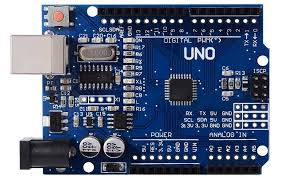
\includegraphics[width=0.4\textwidth , height=  40mm]{arduino_uno}
	\label{fig:arduino_uno}	
\end{wrapfigure}


%\vspace{10mm}
%\hspace{5mm}


La placa de desarrollo, arduino UNO(ver figura \ref{fig:arduino_uno} es una placa de desarrollo basada en hardware y software libre. Está pensada para desarrollos y prototipos rápidos, y posee un entorno de desarrollo integrado, el cual viene preparado para cargar el software dentro de él. Su lenguaje de programación es C/C++. Todos los esquemáticos, y software están disponibles en Internet. Se basa en el microcontrolador AtMega328P.  

Un punto a favor de esta placa de desarrollo, es que poseen librerías para el manejo de los puertos SPI e I2C. En particular, existen librerías para el manejo del display mediante el uso de I2C y el chip ethernet W5100 de manera nativa, es decir, sin necesidad de instalar o descargar ninguna librería adicional. Posee disponibilidad de pines,  y puertos PWM. También posee conversores analógicos digitales. La documentación disponible, se encuentra en su sitio oficial, de manera ordenada. 
La información no oficial, es decir, en Internet es abundante, y existen varios millones de proyectos basados en el ecosistema Arduino dentro de uno de los repositorios más grandes de software: GitHub.    

\subsubsection{STM32VL discovery}
% figura stm32-vl discovery  

\begin{wrapfigure}[12]{l}[10mm]{0.5\textwidth}
	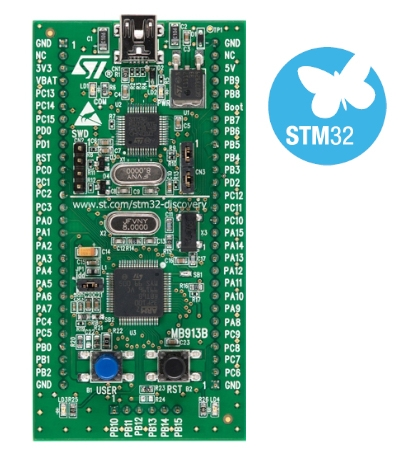
\includegraphics[width=0.4\textwidth,height=45mm] {stm32vl}
	\caption{Placa STM32VLDISCOVERY disponible en el IAR}
	\label{fig:stm32}
\end{wrapfigure}

Esta placa de desarrollo, es desarrollada por la empresa STMicroelectronics. Según la información oficial de su página, esta placa está pensada para el aprendizaje del microcontrolador STM32F100. Este microcontrolador es el núcleo de esta placa,es un procesador con arquitectura ARM. Tiene 64 pines disponibles, varios conversores analógicos digitales. Tiene ejemplos y disponibilidad de software en forma gratuita. No posee documentación sobre la construcción de la placa. Existe muy poca información por fuera de la documentación oficial. Existen algunos foros de sistemas embebidos, pero la discusión es muy escasa, y en general se encuentra en idioma inglés. La placa se muestra en la figura \ref{fig:stm32}




\subsubsection{Comparación de microcontroladores} 
Dado, que se han analizado las tres placas de desarrollo que están disponibles, se van a comparar sus prestaciones y además su disponibilidad en el mercado local. Esto se realiza, basado en las hojas de datos de cada microcontrolador. Este es necesario, ya qué si el equipo se daña durante el desarrollo, o mediante su uso, puede cambiarse de forma inmediata, sin pérdida de tiempo. Esta comparación se realiza en la siguiente tabla:  

% tabla comparativa 
\renewcommand{\arraystretch}{1.2}
\begin{table}[ht]
\makebox[15cm][c]{
\begin{tabular}{|l|c|c|c|}
	\hline
	\textbf{Nombre de la placa} & Arduino Uno & EDU-CIAA &STM32VLDISCOVERY \\
	\hline 
	\textbf{Microcontrolador} & ATmega328P & ARM Cortex-M4F & STM32F100 \\
	\hline 
	\textbf{Canales ADC} &6 canales -10 bit & 3 canales -10 bit  & 16 canales - 12bit \\ 
	\hline 
	\textbf{Puertos Disponibles } & 15 & 80 & 70 \\ 
	\hline 
	\textbf{Comunicación I2C} & Si & Si &Si \\
	\hline 
	\textbf{Comunicación SPI}  & Si & Si &Si \\ 
	\hline 
	\textbf{Disponibilidad} & Si & No  &No  \\
	\hline 
	\textbf{Precios promedios} & \$1000(disponible en todo el país) &\$5.732({único local})  & \$5100(mercado limitado)  \\ \hline
\end{tabular}
}
\caption{Cuadro comparativo de placas disponibles en el Instituto Argentino de radioastronomía}
\label{tab:comp_mc}
\end{table} 




% Explicar muy bien porque se selecciono el microcontrolador

De la tabla \ref{tab:comp_mc}, la placa seleccionada es la denominada Arduino UNO, ya que posee soluciones de software sobre el display, y soporta el chip ethernet W5100 de manera nativa. Esto, implica que la velocidad de desarrollo es superior a la de las otras placas, ya que no se requieren conocimientos detallados sobre los protocolos. 

Por último, el hardware seleccionado para realizar la segunda fase de esta tesis es el siguiente: 
\begin{enumerate}
	\item Placa de desarrollo o microcontrolador: Arduino UNO 
	\item Interfaz de red: Chip Ethernet W5100 
	\item Interfaz de usuario: Display LCD  
\end{enumerate}

Estos tres componentes, ante cualquier tipo de falla, están disponibles en el mercado local, y esto facilita el seguimiento del proyecto en caso de algún fallo en los componentes de hardware. 


